\documentclass[letterpaper,twocolumn,10pt]{article}
\usepackage{usenix,epsfig,endnotes}
\usepackage{graphicx}

\begin{document}

\date{27\textsuperscript{th} April, 2017}

% Title
\title{\Large \textbf{
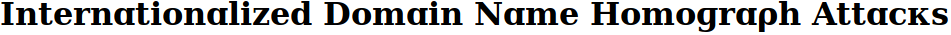
\includegraphics[height=\baselineskip]{title} \\
Project Proposal } \\ \vspace{0.025 in} \large \normalfont
CSE 227: Computer Security - Spring 2017 \\ \textit{
University of California San Diego
}}

% Authors
\author{
{\rm Chen Lai}\\
\normalfont{\texttt{chl588@ucsd.edu}}
\and
{\rm Zhongrong Jian}\\
\normalfont{\texttt{zhjian@ucsd.edu}}
\and
{\rm J. Sidrach}\\
\normalfont{\texttt{jsidrach@ucsd.edu}}
}

\maketitle

\section{What}

Domain names were originally designed to support only ASCII characters.
Internationalized Domain Name (IDN) was proposed back in December 1996 by Martin Dürst for the purpose of letting non-English speaking people use Internet without  additional restrictions.
This extension involves representing Unicode characters in ASCII using Punycode, so that they could be then rendered back into their Unicode representation.
Homograph letters (different letters whose representation is almost, if not, the same), however, present a potential vulnerability.
For example, Cyrillic letter 'a' can look identical to Latin letter 'a' depending on the font.
In other languages, like Chinese, there exists many homograph letters between traditional Chinese and simplified Chinese.
Malicious attackers can then register a domain where one of the letters is actually Cyrillic but whose representation matches a Latin one.
Users could be linked to this newly registered malicious page, and they may not have any visual indication (at least without further interaction) that the page is not the one they think they are visiting.

\section{How}
We will focus our research on the Top 500 Alexa websites, specifically in URL variations where Latin characters are replaced by Cyrillic ones with a similar representation.
By checking and verifying the domain variations, we will classify them into different categories: not registered, owned by the same entity as the original, malicious and unrelated.
We will evaluate the impact of this vulnerability based on the relative percentages we find in the different categories.

On the other hand, browsers also play an important role in defending against IDN homograph attacks.
In this project, the exposure to this vulnerability of different versions of the major browsers will be studied.
We will discuss the solutions implemented by these browsers and their effectiveness, along with some screenshots of the browsers' navigation bar before and after related CVEs were disclosed.
Finally, we will also explore alternative policies, as white/black lists and unconditional rendering, and analyze the possible advantages and drawbacks of each one.

At the end of this project, we will have a statistical evaluation of the current impact of this kind of vulnerability based on the empirical data, so that we can have an idea of the potential impact and the percentage of users at risk.

\section{Potential Issues}
Since we are only collecting data from the Top 500 Alexa websites, the sample size may be too small to find enough illegitimate domain names by just substituting characters by visually equivalent Unicode homoglyphs.
Second, we may need to manually check and classify the illegitimate websites.
This could be a significant time investment if the amount of registered domain names we find by character substitution is high, unless we find a suitable solution to automate the process.

\section{Resources}
We believe that we can perform the empirical study in our own computers, as we will limit the search to the Top 500 Alexa websites.
We also think that we can test different browsers/environments without additional resources.

\end{document}
